\documentclass[UTF8]{ctexart}

% font packages
\usepackage{amsfonts}
\usepackage{amssymb}
\usepackage{amsthm}
\usepackage{amsmath}
\usepackage{mathrsfs}

% margin
\usepackage{geometry}
\geometry{
    paper =a4paper,
    top =3cm,
    bottom =3cm,
    left=2cm,
    right =2cm
}
\linespread{1.2}

% more math operators' support
\usepackage{physics}

% Boldface
\usepackage{bm}

% Tikz
\usepackage{tikz}
\usetikzlibrary{calc}

% Gaussian Elimination
\usepackage{gauss}

% Commutative Graph
\usepackage[all]{xy}

% Comment
\usepackage{comment}

% Colors
\usepackage{xcolor}

% 文字颜色的命令
\newcommand{\tc}[4][white]{{\fcolorbox{#1}{#2}{\textcolor{#3}{#4}}}} % 此命令接受四个参数,第一个参数为边框颜色,默认为白色,第二个参数为文字背景颜色,第三个参数为文字颜色,第四个参数为文字内容。如:\tc[green]{blue}{lime}{Hello,world!}

% Reference support
\usepackage{hyperref}
\hypersetup{
    colorlinks=true,
    linkcolor=blue,
    filecolor=magenta,
    urlcolor=cyan
} % 请在此处自定义链接的颜色,相当于\textcolor

% Info
\title{Title}
\author{Fulcrum4Math}
\date{\today}

% General
\DeclareMathOperator{\N}{\mathbb{N}}                    % Set of Natural Numbers
\DeclareMathOperator{\Z}{\mathbb{Z}}                    % Set of Integers
\DeclareMathOperator{\Q}{\mathbb{Q}}                    % Set of Rational Numbers
\DeclareMathOperator{\R}{\mathbb{R}}                    % Set of Real Numbers
\DeclareMathOperator{\C}{\mathbb{C}}                    % Set of Complex Numbers

\DeclareMathOperator{\Id}{Id}                           % Identity

\DeclareMathOperator{\Ker}{Ker}                         % Kernel of a Homomorphism ($\ker$ is included in package amsmath)
\DeclareMathOperator{\Image}{Im}                        % Image of a mapping

% Mathematical Logic
\DeclareMathOperator{\true}{\mathbb{T}}                    % Tautology
\DeclareMathOperator{\false}{\mathbb{F}}                    % Contradictory Formula
% Set Theory
\DeclareMathOperator{\PP}{\mathcal{P}}                  % Power Sets
\DeclareMathOperator{\card}{card}                       % Cardinality

% Category Theory
\DeclareMathOperator{\Cat}{\mathcal{C}}                 % Category

\DeclareMathOperator{\Hom}{Hom}                         % Set of Homomorphisms
\DeclareMathOperator{\End}{End}                         % Set of Endomorphisms
\DeclareMathOperator{\Aut}{Aut}                         % Set of Automorphisms
\DeclareMathOperator{\Isom}{Isom}                       % Set of Isomorphisms

\DeclareMathOperator{\Ob}{Ob}                           % Objects of a Category
\DeclareMathOperator{\Mor}{Mor}                         % Morphisms of a Category

% Abstract Algebra

\DeclareMathOperator{\stab}{stab}

% Topology
\DeclareMathOperator{\T}{\mathcal{T}}                   % Topology

\DeclareMathOperator{\intr}{int}                        % Interior
\DeclareMathOperator{\cl}{cl}                           % Closure

\DeclareMathOperator{\U}{\overset{\circ}{\mathit{U}}}   % Deleted Neighbourhood

% Linear Algebra

% \rank is included in package physics.
% \tr is included in package physics.

\DeclareMathOperator{\K}{\mathbb{K}}                    % Number Field
\DeclareMathOperator{\F}{\mathbb{F}}                    % Number Field (F)

\DeclareMathOperator{\diag}{\text{diag}}                % Diagonal Matrix
\DeclareMathOperator{\al}{\bm\alpha}                    % Boldfaced vector alpha
\DeclareMathOperator{\bt}{\bm\beta}                     % Boldfaced vector beta
\DeclareMathOperator{\x}{\bm{x}}                        % Boldfaced vector x
\DeclareMathOperator{\0}{\mathbf{0}}                    % Boldfaced vector x

\newcommand{\Jd}[2]{\mathrm{J}_{#1}{(#2)}}              % Jordan Blocks

% \DeclareMathOperator{\A}{\bm{A}}                    % Boldfaced matrix A
% \DeclareMathOperator{\B}{\bm{B}}                    % Boldfaced matrix B
% \DeclareMathOperator{\Cc}{\bm{C}}                   % Boldfaced matrix C

\DeclareMathOperator{\CCol}{Col}                        % Column Space
\DeclareMathOperator{\RRow}{Row}                        % Row Space
\DeclareMathOperator{\Null}{Null}                       % Null Space
\DeclareMathOperator{\rmT}{\mathrm{T}}                  % Transpose

\newcommand{\spn}{\mathrm{span}\text{ }}             % Span
% The original command `\span` leads to the environment `align` misdirected.

\DeclareMathOperator{\adj}{adj}                         % adj Matrix

\newcommand{\GL}[2]{\mathrm{GL}_{#1}(#2)}               % General Linear Group
\newcommand{\SL}[2]{\mathrm{SL}_{#1}(#2)}               % Special Linear Group

\DeclareMathOperator{\lcm}{lcm}                         % LCM

\newcommand{\<}{\langle}                                
\renewcommand{\>}{\rangle}                              % These two for ordinary Hilbert Inner Products <x,y>
\newcommand{\inprod}[2]{\<#1,#2\>}    % Using $\expval{#1}$ (Included in package physics) can replace \<#1\>.
\newcommand{\ocinterval}[2]{\left(#1,#2\right]}
\newcommand{\cointerval}[2]{\left[#1,#2\right)}
\newcommand{\ccinterval}[2]{\left[#1,#2\right]}
\newcommand{\oointerval}[2]{\left(#1,#2\right)}

% Mathematical Analysis

\DeclareMathOperator*{\ulim}{\overline{\lim}}
\DeclareMathOperator*{\llim}{\underline{\lim}}
\newcommand{\diff}[3]{\left. #1 \right|_{#2}^{#3}}    % This command can be replaced by $\eval{#1}_{#2}^{#3}$ in package physics.

\newcommand{\Ball}[2]{\mathcal{B}\left(#1,#2\right)}	% Open Ball

% Theorem template below copied from https://zhuanlan.zhihu.com/p/763738880

% ————————————————————————————————————自定义颜色————————————————————————————————————
\definecolor{dfn_green1}{RGB}{0, 156, 39} % 深绿
\definecolor{dfn_green2}{RGB}{214, 254, 224} % 浅绿

\definecolor{thm_blue1}{RGB}{0, 91, 156} % 深蓝
\definecolor{thm_blue2}{RGB}{218, 240, 255} % 浅蓝

\definecolor{ppt_pink1}{RGB}{172, 0, 175} % 深粉
\definecolor{ppt_pink2}{RGB}{255, 237, 255} % 浅粉

\definecolor{crl_orange1}{RGB}{225, 124, 0} % 深橙
\definecolor{crl_orange2}{RGB}{255, 235, 210} % 浅橙

\definecolor{xmp_purple1}{RGB}{119, 0, 229} % 深紫
\definecolor{xmp_purple2}{RGB}{239, 223, 255} % 浅紫

\definecolor{cxmp_red1}{RGB}{211, 0, 35} % 深红
\definecolor{cxmp_red2}{RGB}{255, 214, 220} % 浅红

\definecolor{prf_grey1}{RGB}{120, 120, 120} % 深灰
\definecolor{prf_grey2}{RGB}{233, 233, 233} % 浅灰

\definecolor{axm_yellow1}{RGB}{192, 192, 0} % 深黄
\definecolor{axm_yellow2}{RGB}{255, 255, 172} % 浅黄

% 将RGB换为rgb,颜色数值取值范围改为0到1
% ————————————————————————————————————自定义颜色————————————————————————————————————

% ————————————————————————————————————盒子设置————————————————————————————————————

\usepackage{tcolorbox} % 盒子效果
\tcbuselibrary{most} % tcolorbox宏包的设置,详见宏包说明文档

% tolorbox提供了tcolorbox环境,其格式如下:
% 第一种格式:\begin{tcolorbox}[colback=⟨背景色⟩, colframe=⟨框线色⟩, arc=⟨转角弧度半径⟩, boxrule=⟨框线粗⟩]   \end{tcolorbox}
% 其中设置arc=0mm可得到直角;boxrule可换为toprule/bottomrule/leftrule/rightrule可分别设置对应边宽度,但是设置为0mm时仍有细边,若要绘制单边框线推荐使用第二种格式
% 方括号内加上title=⟨标题⟩, titlerule=⟨标题背景线粗⟩, colbacktitle=⟨标题背景线色⟩可为盒子加上标题及其背景线
% 第二种格式:\begin{tcolorbox}[enhanced, colback=⟨背景色⟩, boxrule=0pt, frame hidden, borderline={⟨框线粗⟩}{⟨偏移量⟩}{⟨框线色⟩}]   {\end{tcolorbox}}
% 将borderline换为borderline east/borderline west/borderline north/borderline south可分别为四边添加框线,同一边可以添加多条
% 加入breakable属性可以支持盒子拆分到两页中。
% 偏移量为正值时,框线向盒子内部移动相应距离,负值反之

\newenvironment{dfn_box}{
    \begin{tcolorbox}[enhanced, colback=dfn_green2, boxrule=0pt, frame hidden,
        borderline west={0.7mm}{0.1mm}{dfn_green1},breakable]
    }
    {\end{tcolorbox}}
    
\newenvironment{thm_box}{
    \begin{tcolorbox}[enhanced, colback=thm_blue2, boxrule=0pt, frame hidden,
        borderline west={0.7mm}{0.1mm}{thm_blue1},breakable]
    }
    {\end{tcolorbox}}
    
\newenvironment{ppt_box}{
    \begin{tcolorbox}[enhanced, colback=ppt_pink2, boxrule=0pt, frame hidden,
        borderline west={0.7mm}{0.1mm}{ppt_pink1},breakable]
    }
    {\end{tcolorbox}}
    
\newenvironment{crl_box}{
    \begin{tcolorbox}[enhanced, colback=crl_orange2, boxrule=0pt, frame hidden,
        borderline west={0.7mm}{0.1mm}{crl_orange1},breakable]
    }
    {\end{tcolorbox}}
    
\newenvironment{xmp_box}{
    \begin{tcolorbox}[enhanced, colback=xmp_purple2, boxrule=0pt, frame hidden,
        borderline west={0.7mm}{0.1mm}{xmp_purple1},breakable]
    }
    {\end{tcolorbox}}
    
\newenvironment{cxmp_box}{
    \begin{tcolorbox}[enhanced, colback=cxmp_red2, boxrule=0pt, frame hidden,
        borderline west={0.7mm}{0.1mm}{cxmp_red1},breakable]
    }
    {\end{tcolorbox}}
    
\newenvironment{prf_box}{
    \begin{tcolorbox}[enhanced, colback=prf_grey2, boxrule=0pt, frame hidden,
        borderline west={0.7mm}{0.1mm}{prf_grey1},breakable]
    }
    {\end{tcolorbox}}
    
\newenvironment{axm_box}{
    \begin{tcolorbox}[enhanced, colback=axm_yellow2, boxrule=0pt, frame hidden,
        borderline west={0.7mm}{0.1mm}{axm_yellow1},breakable]
    }
    {\end{tcolorbox}}

% tcolorbox宏包还提供了\tcbox指令,用于生成行内盒子,可制作高光效果

        % \newcommand{\hl}[1]{
        %     \tcbox[on line, arc=0pt, colback=hlan!5!white, colframe=hlan!5!white, boxsep=1pt, left=1pt, right=1pt, top=1.5pt, bottom=1.5pt, boxrule=0pt]
        % {\bfseries \color{hlan}#1}}

% 其中on line将盒子放置在本行(缺失会跳到下一行),boxsep用于控制文本内容和边框的距离,left、right、top、bottom则分别在boxsep的参数的基础上分别控制四边距离

% ————————————————————————————————————盒子设置————————————————————————————————————

% ————————————————————————————————————定理类环境设置————————————————————————————————————
\newtheoremstyle{MyStyle}{0pt}{}{}{\parindent}{\bfseries}{}{1em}{} % 定义新定理风格。格式如下:
%\newtheoremstyle{⟨风格名⟩}
%                {⟨上方间距⟩} % 若留空,则使用默认值
%                {⟨下方间距⟩} % 若留空,则使用默认值
%                {⟨主体字体⟩} % 如 \itshape
%                {⟨缩进长度⟩} % 若留空,则无缩进;可以使用 \parindent 进行正常段落缩进
%                {⟨定理头字体⟩} % 如 \bfseries
%                {⟨定理头后的标点符号⟩} % 如点号、冒号
%                {⟨定理头后的间距⟩} % 不可留空,若设置为 { },则表示正常词间间距;若设置为 {\newline},则环境内容开启新行
%                {⟨定理头格式指定⟩} % 一般留空
% 定理风格决定着由 \newtheorem 定义的环境的具体格式,有三种定理风格是预定义的,它们分别是:
% plain: 环境内容使用意大利斜体,环境上下方添加额外间距
% definition: 环境内容使用罗马正体,环境上下方添加额外间距
% remark: 环境内容使用罗马正体,环境上下方不添加额外间距

\theoremstyle{MyStyle} % 设置定理风格 

% 定义定义环境,格式为\newtheorem{⟨环境名⟩}{⟨定理头文本⟩}[⟨上级计数器⟩]或\newtheorem{⟨环境名⟩}[⟨共享计数器⟩]{⟨定理头文本⟩},其变体\newtheorem*不带编号

% 以下的每个环境接受参数,请按顺序填入:
% #1 环境标题(中文)

\newtheorem{axiom}{公理}[section]
\newenvironment{axm}[2]
{
    \begin{axm_box}
        \begin{axiom}
            \textbf{#1
                \ifx\relax#2\relax\else % 检查 #2 是否为空
                    (#2) % 如果 #2 不为空,渲染 [空格](#2)
                \fi}
            \newline
}
{
        \end{axiom}
    \end{axm_box}
}

\newtheorem{definition}{定义}[subsection]
\newenvironment{dfn}[2]
{
    \begin{dfn_box}
        \begin{definition}
            \textbf{#1
                \ifx\relax#2\relax\else % 检查 #2 是否为空
                    (#2) % 如果 #2 不为空,渲染 [空格](#2)
                \fi}
            \newline
}
{
        \end{definition}
    \end{dfn_box}
}

\newtheorem{concept}[definition]{概念}
\newenvironment{cpt}[1]
{
    \begin{dfn_box}
        \begin{concept}
            \textbf{#1}
            \newline
}
{
        \end{concept}
    \end{dfn_box}
}

\newtheorem{syntax}[definition]{语法}
\newenvironment{syn}[1]
{
    \begin{thm_box}
        \begin{syntax}
            \textbf{#1}
            \newline
}
{
        \end{syntax}
    \end{thm_box}
}

\newtheorem{theorem}[definition]{定理}
\newenvironment{thm}[2]
{
    \begin{thm_box}
        \begin{theorem}
            \textbf{#1
                \ifx\relax#2\relax\else % 检查 #2 是否为空
                    (#2) % 如果 #2 不为空,渲染 [空格](#2)
                \fi}
            \newline
}
{
        \end{theorem}
    \end{thm_box}
}

\newtheorem{mytactic}{策略}
\newenvironment{tactic}[1]
{
    \begin{thm_box}
        \begin{mytactic}
            \textbf{#1}
            \newline
}
{
        \end{mytactic}
    \end{thm_box}
}

\newtheorem{myvariation}{Tactic 变体}[definition]
\newenvironment{tacticvar}[1]
{
    \begin{ppt_box}
        \begin{myvariation}
            \textbf{#1}
            \newline
}
{
        \end{myvariation}
    \end{ppt_box}
}

\newtheorem{example}{ 例\, }[subsection]
\newenvironment{xmp}[1]
{
    \begin{xmp_box}
        \begin{example}
            \textbf{#1}
            \newline
}
{
        \end{example}
    \end{xmp_box}
}

\newtheorem{cexample}{反例}[subsection]
\newenvironment{cxmp}[1]
{
    \begin{cxmp_box}
        \begin{cexample}
            \textbf{#1}
            \newline
}
{
        \end{cexample}
    \end{cxmp_box}
}

\newtheorem*{myproof}{证明: \newline}
\newenvironment{prf}{\begin{prf_box}\begin{myproof}}{\end{myproof}\end{prf_box}}

\newenvironment{crs}[4]
{
    \begin{thm_box}
        \textbf{课程 #1: #2}
        
        \ifx\relax#3\relax\else % 检查 #3 是否为空
            \textbf{主讲: }#3 % 如果 #3 不为空,渲染 [空格](#3)
        \fi
        
        \ifx\relax#4\relax\else % 检查 #4 是否为空
            \textbf{课程材料: }#4 % 如果 #4 不为空,渲染 [空格](#4)
        \fi

        \textbf{主要内容: }
}
{
    \end{thm_box}
}

\newtheorem{project}{课题}
\newenvironment{prj}[1]
{
    \begin{xmp_box}
        \begin{project}
            \textbf{#1}
            \newline
}
{
        \end{project}
    \end{xmp_box}
}

\usepackage{listings}
\newcommand{\smallsec}[1]{\paragraph{#1.}}
\lstset{
    basicstyle = \ttfamily,
}

% Define Colors: 
\definecolor{leanblue}{RGB}{0,0,255}
\colorlet{keyword}{leanblue}
\colorlet{punct}{leanblue}

\definecolor{sorry}{RGB}{255,0,0}
\definecolor{comment}{RGB}{0,128,0}
\definecolor{string}{RGB}{163,21,21}
\definecolor{num}{RGB}{9,134,88}

\definecolor{thname}{RGB}{121,94,38}

\definecolor{background}{HTML}{EEEEEE}
\definecolor{delim}{RGB}{20,105,176}

\newcommand*{\lean}[1]{\texttt{\color{blue}#1}}

\lstdefinelanguage{lean}{
    % Define Keywords: 
    alsoletter = {\#,\?,*,.},
    keywords = {
        import, 
        namespace, 
        open, 
        variable, 
        Prop, 
        Type, 
        Type*, 
        % Declarations: 
        protected, 
        class, 
        where, 
        export, 
        instance, 
        infix, 
        def, 
        axiom, 
        example, 
        theorem, 
        lemma, 
        fun, 
        by, 
        % Basics: 
        \#check, 
        \#leansearch, 
        \#eval, 
        % Tactics: 
        exact, 
            % FOL: 
            intro,
            intros, 
            rintro, 
            apply,
            apply?, 
            constructor, 
            rcases, 
            obtain, 
            use, 
            left, 
            right, 
            cases, 
            case, 
            by\_cases, 
            by\_contra, 
            contrapose, 
            contrapose!,
            % Others: 
            symm, 
            calc, 
            unfold, 
            have, 
            let, 
            rw, 
            at, 
            change, 
            show, 
            ring, 
            simp, 
            rfl, 
        }, 
    keywords = [2]{sorry}, 
    %
    numbers=left,
    numberstyle=\color{num},
    %
    % morecomment = [l]{--},
    moredelim=[l][\color{comment}]{--}, % morecomment -> moredelim, so that Unicode characters can be used in comments. 
    moredelim=[is][\color{thname}]{\#tm\{}{\}}, 
    moredelim=[is][\color{leanblue}]{\\lean\{}{\}}, 
    morecomment = [s]{/-}{-/},
    commentstyle = \color{comment}, 
    moredelim=[s][\color{string}]{"}{"}, 
    %
    stringstyle = \color{string}, 
    %
    stepnumber=1,
    numbersep=8pt,
    showstringspaces=false,
    breaklines=true,
    frame=lines,
    backgroundcolor=\color{background},
    literate=
    % Keywords
        {th\_name}{{{\color{thname}th\_name}}}{6}
    % Math Symbols
        {ℕ}{{\ensuremath{\mathbb{N}}}}{1}
        {ℤ}{{\ensuremath{\mathbb{Z}}}}{1}
        {ℝ}{{\ensuremath{\mathbb{R}}}}{1}
        {ℚ}{{\ensuremath{\mathbb{Q}}}}{1}
        {ℂ}{{\ensuremath{\mathbb{C}}}}{1}
        {∩}{{\ensuremath{\cap}}}{1}
        {∪}{{\ensuremath{\cup}}}{1}
        {⊂}{{\ensuremath{\subseteq}}}{1}
        {⊆}{{\ensuremath{\subseteq}}}{1}
        {⊄}{{\ensuremath{\nsubseteq}}}{1}
        {⊈}{{\ensuremath{\nsubseteq}}}{1}
        {⊃}{{\ensuremath{\supseteq}}}{1}
        {⊇}{{\ensuremath{\supseteq}}}{1}
        {⊅}{{\ensuremath{\nsupseteq}}}{1}
        {⊉}{{\ensuremath{\nsupseteq}}}{1}
        {∈}{{\ensuremath{\in}}}{1}
        {∉}{{\ensuremath{\notin}}}{1}
        {∋}{{\ensuremath{\ni}}}{1}
        {∌}{{\ensuremath{\notni}}}{1}
        {∅}{{\ensuremath{\emptyset}}}{1}
        {∫}{{\ensuremath{\int}}}{1}
        {∑}{{\ensuremath{\mathrm{\Sigma}}}}{1}
        {Π}{{\ensuremath{\mathrm{\Pi}}}}{1}
        {≤}{{\ensuremath{\leq}}}{1}
        {≥}{{\ensuremath{\geq}}}{1}
        {≠}{{\ensuremath{\neq}}}{1}
        {≈}{{\ensuremath{\approx}}}{1}
        {≡}{{\ensuremath{\equiv}}}{1}
        {≃}{{\ensuremath{\simeq}}}{1}
    % Greek Letters lowercase
        {α}{{\ensuremath{\mathrm{\alpha}}}}{1}
        {β}{{\ensuremath{\mathrm{\beta}}}}{1}
        {γ}{{\ensuremath{\mathrm{\gamma}}}}{1}
        {δ}{{\ensuremath{\mathrm{\delta}}}}{1}
        {ε}{{\ensuremath{\mathrm{\varepsilon}}}}{1}
        {ζ}{{\ensuremath{\mathrm{\zeta}}}}{1}
        {η}{{\ensuremath{\mathrm{\eta}}}}{1}
        {θ}{{\ensuremath{\mathrm{\theta}}}}{1}
        {ι}{{\ensuremath{\mathrm{\iota}}}}{1}
        {κ}{{\ensuremath{\mathrm{\kappa}}}}{1}
        {μ}{{\ensuremath{\mathrm{\mu}}}}{1}
        {ν}{{\ensuremath{\mathrm{\nu}}}}{1}
        {ξ}{{\ensuremath{\mathrm{\xi}}}}{1}
        {π}{{\ensuremath{\mathrm{\mathnormal{\pi}}}}}{1}
        {ρ}{{\ensuremath{\mathrm{\rho}}}}{1}
        {σ}{{\ensuremath{\mathrm{\sigma}}}}{1}
        {τ}{{\ensuremath{\mathrm{\tau}}}}{1}
        {φ}{{\ensuremath{\mathrm{\varphi}}}}{1}
        {χ}{{\ensuremath{\mathrm{\chi}}}}{1}
        {ψ}{{\ensuremath{\mathrm{\psi}}}}{1}
        {ω}{{\ensuremath{\mathrm{\omega}}}}{1}
    % Greek Letters UPPERCASE
        {Γ}{{\ensuremath{\mathrm{\Gamma}}}}{1}
        {Δ}{{\ensuremath{\mathrm{\Delta}}}}{1}
        {Θ}{{\ensuremath{\mathrm{\Theta}}}}{1}
        {Λ}{{\ensuremath{\mathrm{\Lambda}}}}{1}
        {Σ}{{\ensuremath{\mathrm{\Sigma}}}}{1}
        {Φ}{{\ensuremath{\mathrm{\Phi}}}}{1}
        {Ξ}{{\ensuremath{\mathrm{\Xi}}}}{1}
        {Ψ}{{\ensuremath{\mathrm{\Psi}}}}{1}
        {Ω}{{\ensuremath{\mathrm{\Omega}}}}{1}
    % Arrows
        {↦}{{\ensuremath{\mapsto}}}{1}
        {←}{{\ensuremath{\leftarrow}}}{1}
        {<-}{{\ensuremath{\leftarrow}}}{1}
        {→}{{\ensuremath{\rightarrow}}}{1}
        {->}{{\ensuremath{\rightarrow}}}{1}
        {↔}{{\ensuremath{\leftrightarrow}}}{1}
        {<->}{{\ensuremath{\leftrightarrow}}}{1}
        {⇒}{{\ensuremath{\Rightarrow}}}{1}
        {⟹}{{\ensuremath{\Longrightarrow}}}{1}
        {⇐}{{\ensuremath{\Leftarrow}}}{1}
        {⟸}{{\ensuremath{\Longleftarrow}}}{1}
        {Σ}{{\ensuremath{\Sigma}}}{1}
        {Π}{{\ensuremath{\Pi}}}{1}
        {∀}{{\ensuremath{\forall}}}{1}
        {∃}{{\ensuremath{\exists}}}{1}
        {λ}{{\ensuremath{\mathrm{\lambda}}}}{1}
        {∧}{{\ensuremath{\wedge}}}{1}
        {∨}{{\ensuremath{\vee}}}{1}
        {¬}{{\ensuremath{\neg}}}{1}
        {⊢}{{\ensuremath{\vdash}}}{1}
        {‖}{{\ensuremath{\|}}}{1}
    % subscripts
        {₁}{{\ensuremath{_1}}}{1}
        {₂}{{\ensuremath{_2}}}{1}
        {₃}{{\ensuremath{_3}}}{1}
        {₄}{{\ensuremath{_4}}}{1}
        {₅}{{\ensuremath{_5}}}{1}
        {₆}{{\ensuremath{_6}}}{1}
        {₇}{{\ensuremath{_7}}}{1}
        {₈}{{\ensuremath{_8}}}{1}
        {₉}{{\ensuremath{_9}}}{1}
        {₀}{{\ensuremath{_0}}}{1}
        {ᵢ}{{\ensuremath{_i}}}{1}
        {ⱼ}{{\ensuremath{_j}}}{1}
        {ₐ}{{\ensuremath{_a}}}{1}
        {⁻¹}{{\ensuremath{^{-1}}}}{1}
        {¹}{{\ensuremath{^1}}}{1}
        {ₙ}{{\ensuremath{_n}}}{1}
        {ₘ}{{\ensuremath{_m}}}{1}
        {ₚ}{{\ensuremath{_p}}}{1}
        {ᶜ}{{\ensuremath{^{\mathrm{C}}}}}{1}
    % Others
        {↑}{{\ensuremath{\uparrow}}}{1}
        {↓}{{\ensuremath{\downarrow}}}{1}
        {⊢}{{\ensuremath{\vdash}}}{1}
        {|-}{{\ensuremath{\vdash}}}{1}
        {⊥}{{\ensuremath{\perp}}}{1}
        {∞}{{\ensuremath{\infty}}}{1}
        {∂}{{\ensuremath{\partial}}}{1}
        {√}{{\ensuremath{\sqrt}}}{1}
        {∘}{{\ensuremath{\circ}}}{1}
        {×}{{\ensuremath{\times}}}{1}
        {∆}{{\ensuremath{\triangle}}}{1}
        {⟨}{{\ensuremath{\color{leanblue}\langle}}}{1}
        {⟩}{{\ensuremath{\color{leanblue}\rangle}}}{1}
        {⦃}{{\ensuremath{\color{leanblue}\{\![}}}{1}
        {⦄}{{\ensuremath{\color{leanblue}]\!\}}}}{1}
        {ℒ}{{\ensuremath{\mathscr{L}}}}{1}
        {𝒫}{{\ensuremath{\mathcal{P}}}}{1}
        {·}{{\ensuremath{\cdot}}}{1},
}

\lstdefinestyle{lean}{
    language=lean,
    numbers=none, 
    keywordstyle=\color{leanblue},
    keywordstyle=[2]\color{sorry},
    % frame=none,
    backgroundcolor=\color{white}, 
}

\newcommand{\Goal}{\texttt{\,\color{leanblue}\ensuremath{\vdash}\,}}


\begin{document}
    \begin{center}
        {\LARGE\textbf{2025 Lean 与数学形式化讲义(2B)}}

        上海交通大学 AI4MATH 团队
    \end{center}

    \setcounter{section}{2}
    \section{朴素集合论}

    \subsection{定义与定理}


    \begin{tactic}
        {\lean{unfold}}
        \lean{unfold} 策略可以将对象展开为其定义. 其实通常不影响证明, 但是会方便我们观察对象的定义. 

        \begin{lstlisting}[style=lean]
    def a : Prop := sorry
    def b : Prop := sorry
    theorem b_of_a : a → b := by sorry

    def A : Prop := a
    def B : Prop := b
    theorem th_name : A → B := by
      unfold A B
      exact b_of_a

    theorem #tm{th_name2} : A → B := by
      intro hA
      have : a := Iff.rfl.mp hA
      have : b := b_of_a this
      have : B := Iff.rfl.mpr this
      exact this

    theorem #tm{th_name3} : a → b := b_of_a
    -- Iff.rfl and unfold tactic in fact does nothing. 
        \end{lstlisting}
    
    在任何一个新定义被引入之初, 我们很少有工具能处理它, 此时大部分基本性质都通过还原概念的定义, 借助已成熟的理论框架证明. 而当一个成熟的概念已有诸多相关定理时, 便可直接使用已有定理. 
    \[
    \xymatrix{
        \text{较高级的概念} & & A\ar@{<->}[d]_{\texttt{rfl}}\ar[r]^{\texttt{h}} & B\ar@{<->}[d]^{\texttt{rfl}} & \text{更高层次定理的证明} h\\
        \text{较原始的概念}\ar[u]^{\text{定义封装}} & & a\ar[r]^{\texttt{h'}} & b & \text{通过基本定理的证明合成证明} h'\ar[u]_{\text{相当于}}
    }
    \]
    \end{tactic}

    \begin{xmp}
        {展开定义}
        使用 \lean{unfold} 策略展开定义, 方便我们查看定义的内容并用定义来证明命题. 
        \begin{lstlisting}[style=lean]
    def #tm{f} (n : ℕ) : ℕ := n + 1
    theorem th_name (n : ℕ) : f n = n + 1 := by
      unfold f          -- Goal: n + 1 = n + 1
      rfl               -- No Goals
        \end{lstlisting}
    \end{xmp}

    \subsection{Mathlib 简介}

        大家应该或多或少在中学和本科的数学考试中遇到过``这个结论要不要证''的问题. 在数学考试中, 通常有一个设定的考核大纲, 其中一些主干的命题是教科书上已经证明的, 作为考试题目的命题被视为是还没有证明的, 而一些``二级结论''可能介于二者之间, 是否要为这些命题提供证明往往成为阅卷人和考生争议不休的问题. 这种情况主要源于中学和本科的数学考试的内容往往是人类几个世纪前早已建立的理论框架. 在数学研究中, 为了创造新的数学, 所有已被证明的数学均可为我们所用. 但是有一个问题始终存在: 我们有哪些命题的证明? 

        我们之前已经讲过, Lean 中借助已有结论证明定理等同于用已有命题的证明对象合成出新的命题的证明对象, 那么问题就变成了: 哪里存储了我们已有的证明. 对于 Lean 来说, 我们有一个社区维护的标准库, 即 Mathlib\footnote{关于 Mathlib 的详细信息请关注 Lean 社区主页或 Github 项目主页: https://github.com/leanprover-community/mathlib4}. 
        
        有许多可视化工具可以直观地感受 Mathlib 库的规模和其中复杂的关系, 例如 Mathlib Explorer\footnote{Github 项目地址: https://github.com/Crispher/MathlibExplorer; 视频介绍: https://www.bilibili.com/video/BV1ex4y1r7tA}: 
        
        \begin{figure}[htbp]
            \centering
            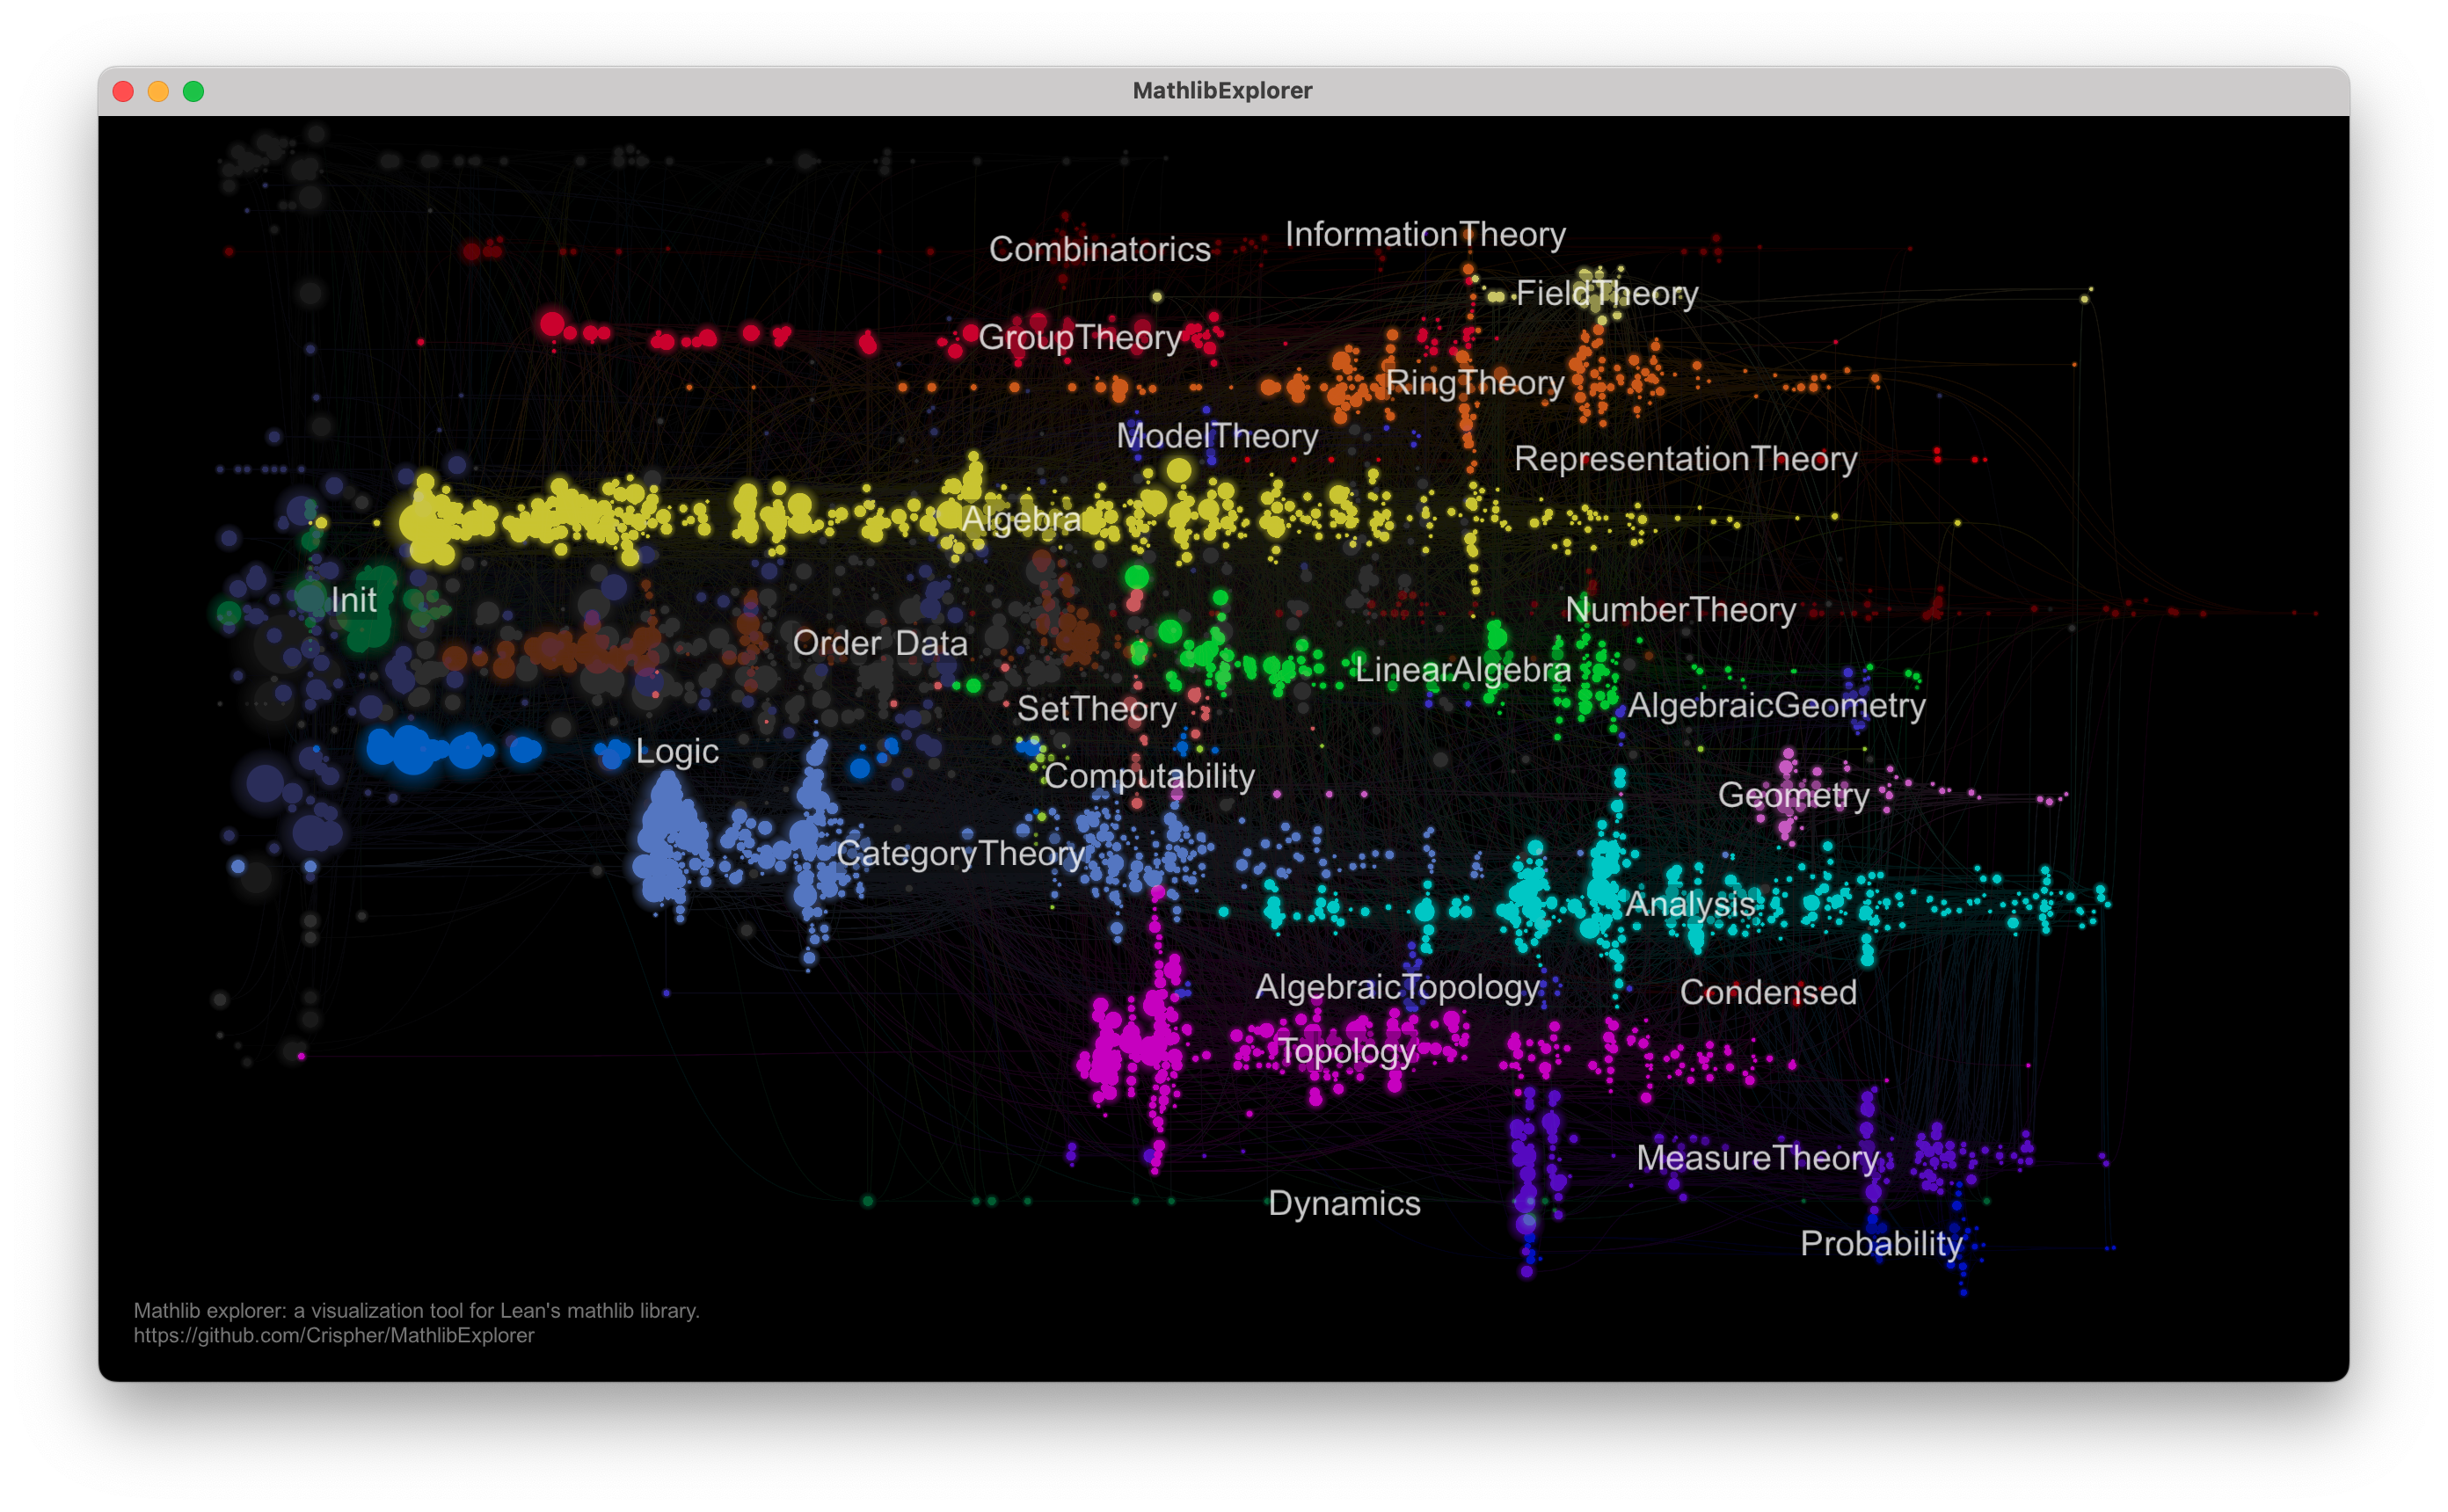
\includegraphics[width=\textwidth]{figures/MathlibExplorer.png}\label{fig:MathlibExplorer}
            \caption{Mathlib Explorer 页面}
        \end{figure}

        图中每一个节点是 Mathlib 中的一个文件, 可以理解为一系列相近概念的集合. 节点之间通过连线刻画各个文件之间的依赖关系, 最左侧是最底层的数学基础, 右侧的概念依赖左侧概念建立. 
        
        Mathlib 中有逾 20 万个条目, 却仍然有诸多还未覆盖的数学领域以及各种缺陷. 在证明过程中使用 Mathlib 中的已有结论实在不是一件容易的事. 好在我们有一些方法来更加方便地查找和使用 Mathlib: 

    \subsection{查找 Mathlib 中的内容}

        查找 Mathlib 中定理最基本的方式当然是直接查阅 Mathlib 库源代码. 如果要使用 Lean 进行特定领域的研究, 我们可能需要熟读相关领域的 Mathlib 源代码以了解一些常用结论的位置, 或是通过 \texttt{Ctrl + Click} 跳转至一些概念的定义, 尝试从上下文和相邻文档中查找所需的定理. 目前 Mathlib 库缺乏简明易懂的自然语言文档\footnote{自动生成的 Lean 官方文档: https://leanprover-community.github.io/mathlib4\_docs/index.html}, 这导致学习的成本十分高昂. 

        另一种方法是通过 Mathlib 中定理证明对象的变量命名习惯\footnote{Mathlib 命名习惯: https://leanprover-community.github.io/contribute/naming.html}, 反向猜测所需命题证明的变量名, 借助 VS Code 的自动补全功能 (可通过 \texttt{Ctrl + Space}打开) 来查找. 

        \begin{xmp}
            {Mathlib 中的定理命名习惯}
            一般严格小于号 $<$ 用 \texttt{lt} 表示, 而小于等于号 $\leq$ 用 \texttt{le} 表示, 函数类型用 \texttt{of} 表示, 算子之间用下滑线 \texttt{\_} 连接, 于是我们有: \footnote{这里算子的顺序是: Goal, Arg1, Arg2, 以此类推}
            \begin{lstlisting}[style=lean]
    #check lt_of_le_of_lt       -- ... , a ≤ b → b < c → a < c
    #check lt_of_lt_of_le       -- ... , a < b → b ≤ z → a < z
    #check le_of_lt             -- ... , a < b → a ≤ b
            \end{lstlisting}
        \end{xmp}

        在策略证明环境中, 可以使用 \lean{apply?} 策略: 
        
        \begin{tactic}
            {\lean{apply?}}
            在策略证明中使用 \lean{apply?} 策略, 会返回一系列可用的证明步骤和剩余目标供选择: 
            \begin{lstlisting}[style=lean]
    theorem th_name : /- proposition -/ := by
      apply?        -- suggestions: ...
      sorry
            \end{lstlisting}
        \end{tactic}

        定理查找方面最显著的成果当属定理查找器. 稍早的成果有 Moogle, 但并未开源; 北京大学团队开发了 LeanSearch\footnote{https://arxiv.org/pdf/2403.13310} 工具用于 Mathlib 库的查找. LeanSearch 有两种使用方法, 可以通过网页版\footnote{https://leansearch.net/}直接使用: 或是通过 Lean 内置的 \lean{\#leansearch} 命令查询: 

        \begin{syn}
            {\lean{\#leansearch}}
            使用 \lean{\#leansearch} 命令可以搜索 Mathlib 
            \begin{lstlisting}[style=lean]
    #leansearch "For integers a and b, if a + b = 0, then a = -b."
        -- LeanSearch Search Results: 
        -- 1. ...
        -- 2. ...
            \end{lstlisting}

            类似的命令还有 \lean{\#moogle}, \lean{\#loogle} 等. 
        \end{syn}
        
        \begin{figure}[htbp]
            \centering
            \includegraphics[width=0.4\textwidth]{figures/Leansearch1.png}\label{fig:LeanSearch1}
            $\qquad$
            \includegraphics[width=0.4\textwidth]{figures/Leansearch2.png}\label{fig:LeanSearch2}
            \caption{LeanSearch 工作原理 (图片引自 LeanSearch 论文\textit{A Semantic Search Engine for Mathlib4})}
        \end{figure}

        LeanSearch 借由 Mathlib 库代码, 对象之间的依赖关系和 Mathlib 文档注释生成提示词提交大语言模型, 递归地对 Mathlib 代码进行非形式化得到各个条目的自然语言描述, 再通过嵌入模型 (Embedding) 将自然语言转化为高维向量, 与由用户输入并经大语言模型增强过后的查询语句嵌入得到的高维向量进行比对, 通过计算余弦距离 (Cosine Distance) 得到与查询语句最为相似的若干个 Mathlib 代码条目. 

        下面我们简单讲解 Mathlib 中朴素集合论的一些基本概念和定理. 由于 Mathlib 的规模实在太大, 我们无法一一介绍, 主要意在让大家对 Mathlib 的使用方法 (即 Lean 的常规使用风格) 有一个大致的概念. 

    \subsection{基本概念}

    \texttt{Mathlib.Data.Set} 中定义的集合与我们常见的 ZFC 公理集合论理论框架不完全相同, 更像是高中学习的朴素集合论, 只是通过类型论元语言规避了悖论. 这种做法也许是 Russell 先生最早提出类型论的初衷. 以下是一些简单定义说明: 
        
        \begin{dfn}
            {类型集合}
            {\texttt{Set}}
            若 $\alpha$ 是一个类型, 定义 $\alpha$ 上的一个一元谓词为一个 \textbf{$\alpha$-集合}, 记作 $\texttt{Set}(\alpha)$: 
            \begin{lstlisting}[style=lean]
    def #tm{Set} (α : Type u) := α → Prop
            \end{lstlisting}
        \end{dfn}

        \begin{dfn}
            {由谓词分离的类型集合}
            {\texttt{setOf}}
            若 $\alpha$ 是一个类型, $p$ 是一个 $\alpha$ 上的一元谓词, 定义由 $\alpha$ 上的一元谓词 $p$ 分离的 $\alpha$ 集合为一元谓词 $p$ 自身, 记作 $\{x : \alpha \mid p(x)\}$: 
            \begin{lstlisting}[style=lean]
    def #tm{setOf} {α : Type u} (p : α → Prop) : Set α := p
            \end{lstlisting}
        \end{dfn}

        \begin{dfn}
            {属于关系}
            {\texttt{Mem}}
            对任何一个类型 $\alpha$, 定义 $\alpha$ 的元素 $a$ 与 $\alpha$-集合 $s$ 满足\textbf{属于关系 (Membership)}, 当且仅当 $a$ 适合一元谓词 $s$, 记作 $a\in s$: 
            \begin{lstlisting}[style=lean]
    protected def #tm{Mem} (s : Set α) (a : α) : Prop := s a

    class #tm{Membership} (α : outParam (Type u)) (γ : Type v) where
      mem : γ → α → Prop

    \lean{notation}:50 a:50 " ∈ " b:50 => Membership.mem b a
    
    instance : Membership α (Set α) := ⟨Set.Mem⟩
            \end{lstlisting}
        \end{dfn}

        \begin{dfn}
            {子集关系}
            {\texttt{Subset}}
            对于 $\alpha$-集合 $s_1, s_2$, 定义 $s_1, s_2$ 满足\textbf{子集关系}当且仅当在 $s_1$ 中的元素总是在 $s_2$中, 记作 $s_1\subseteq s_2$:
            \begin{lstlisting}[style=lean]
    protected def #tm{Subset} (s₁ s₂ : Set α) := ∀ ⦃a⦄, a ∈ s₁ → a ∈ s₂

    class #tm{LE} (α : Type u) where
      le : α → α → Prop

    infix:50 " ≤ "  => LE.le

    instance : LE (Set α) := ⟨Set.Subset⟩

    class #tm{HasSubset} (α : Type u) where
      Subset : α → α → Prop
    export HasSubset (Subset)
    
    infix:50 " ⊆ " => Subset

    instance : HasSubset (Set α) := ⟨(· ≤ ·)⟩
            \end{lstlisting}
        \end{dfn}

        \begin{dfn}
            {空集}
            {\texttt{EmptyCollection}}
            定义为将任意元素映射到 \texttt{False} 的函数, 记作 $\emptyset$ 或 $\{\}$: 
            \begin{lstlisting}[style=lean]
    class #tm{EmptyCollection} (α : Type u) where
      emptyCollection : α

    \lean{notation} "{" "}" => EmptyCollection.emptyCollection
    \lean{notation} "∅"     => EmptyCollection.emptyCollection

    instance : EmptyCollection (Set α) := ⟨fun _ ↦ False⟩
            \end{lstlisting}
        \end{dfn}

        \begin{dfn}
            {宇集}
            {\texttt{univ}}
            一个类型中的所有元素构成的集合称为该类型的\textbf{宇集 (Universe)}, 记作 $\alpha$ 的宇集 $\texttt{univ}(\alpha)$: 
            \begin{lstlisting}[style=lean]
    def #tm{univ} : Set α := {_a | True}
            \end{lstlisting}
        \end{dfn}

        \begin{dfn}
            {插入运算}
            {\texttt{insert}}
            对于 $\alpha$-集合 $s$ 和 $\alpha$ 类型的元素 $a$, 定义将 $a$ 到 $s$ 的\textbf{插入}为 $\{a\}\cup s$: 
            \begin{lstlisting}[style=lean]
    protected def #tm{insert} (a : α) (s : Set α) : Set α
      := {b | b = a ∨ b ∈ s}

    class #tm{Insert} (α : outParam <| Type u) (γ : Type v) where
      insert : α → γ → γ

    instance : Insert α (Set α) := ⟨Set.insert⟩
            \end{lstlisting}
        \end{dfn}

        
        \begin{dfn}
            {单元集}
            {\texttt{singleton}}
            设 $a$ 是一个 $\alpha$ 类型的元素, 定义由 $a$ 生成的单元集为只包含 $a$ 的 $\alpha$-集合, 记作 $\{a\}$:
            \begin{lstlisting}[style=lean]
    protected def #tm{singleton} (a : α) : Set α := {b | b = a}

    class #tm{Singleton} (α : outParam <| Type u) (β : Type v) where
      singleton : α → β
    
    instance instSingletonSet : Singleton α (Set α) := ⟨Set.singleton⟩
            \end{lstlisting}
        \end{dfn}
    
        
        \begin{dfn}
            {并集}
            {\texttt{Union}}
            并集是析取命题的封装, 记作 $\cup$. 
            \begin{lstlisting}[style=lean]
    protected def #tm{union} (s₁ s₂ : Set α) : Set α
      := {a | a ∈ s₁ ∨ a ∈ s₂}

    class #tm{Union} (α : Type u) where
      union : α → α → α

    \lean{infixl}:65 " ∪ " => Union.union
    
    instance : Union (Set α) := ⟨Set.union⟩
            \end{lstlisting}
        \end{dfn}

        
        \begin{dfn}
            {交集}
            {\texttt{Inter}}
            交集是合取命题的封装, 记作 $\cap$. 
            \begin{lstlisting}[style=lean]
    protected def #tm{inter} (s₁ s₂ : Set α) : Set α
      := {a | a ∈ s₁ ∧ a ∈ s₂}
    
    class #tm{Inter} (α : Type u) where
      inter : α → α → α
    
    \lean{infixl}:70 " ∩ " => Inter.inter
    
    instance : Inter (Set α) := ⟨Set.inter⟩
            \end{lstlisting}
        \end{dfn}

        \begin{dfn}
            {补集}
            {\texttt{compl}}
            补集是否定命题的封装, 记作 $^{\mathrm{C}}$.
            \begin{lstlisting}[style=lean]
    protected def #tm{compl} (s : Set α) : Set α := {a | a ∉ s}

    class #tm{HasCompl} (α : Type*) where
      compl : α → α
    export HasCompl (compl)

    \lean{postfix}:1024 "ᶜ" => compl
            \end{lstlisting}
        \end{dfn}
        
        \begin{dfn}
            {差集}
            {\texttt{diff}}
            差集
            \begin{lstlisting}[style=lean]
    protected def #tm{diff} (s t : Set α) : Set α := {a ∈ s | a ∉ t}
    
    class SDiff (α : Type u) where
      sdiff : α → α → α
    
    infix:70 " \\ " => SDiff.sdiff

    instance : SDiff (Set α) := ⟨Set.diff⟩
            \end{lstlisting}
        \end{dfn}
        
        \begin{dfn}
            {幂集}
            {\texttt{powerset}}
            集合的全体子集构成的集合称为该集合的\textbf{幂集 (Powerset)}, $\alpha$-集合 $s$ 的幂集记作 $\mathcal{P}(s)$. 
            \begin{lstlisting}[style=lean]
    def #tm{powerset} (s : Set α) : Set (Set α) := {t | t ⊆ s}
    \lean{prefix}:100 "𝒫" => powerset
            \end{lstlisting}
        \end{dfn}

        \begin{dfn}
            {像集}
            {\texttt{image}}
            设 $\alpha,\beta$ 是类型, $f$ 是从 $\alpha$ 到 $\beta$ 的映射, $s$ 是 $\alpha$-集合, $s$ 全体元素在 $f$ 下的像构成的集合称为 $f$ 的\textbf{像集 (Image)}, 记作 $f(s)$. 
            \begin{lstlisting}[style=lean]
    def image {β : Type v} (f : α → β) (s : Set α) : Set β := {f a | a ∈ s}
    infixl:80 " '' " => image
            \end{lstlisting}
        \end{dfn}

        \begin{dfn}
            {原像集}
            {\texttt{preimage}}
            设 $\alpha,\beta$ 是类型, $f$ 是从 $\alpha$ 到 $\beta$ 的映射, $s$ 是 $\beta$-集合, 映射到 $s$ 的全体元素构成的集合称为 $f$ 的\textbf{原像 (Preimage)}, 记作 $f^{-1}(s)$. 
            \begin{lstlisting}[style=lean]
    def #tm{preimage} (f : α → β) (s : Set β) : Set α := {x | f x ∈ s}
    \lean{infixl}:80 " ⁻¹' " => preimage
            \end{lstlisting}
        \end{dfn}

        \begin{dfn}
            {单射}
            {\texttt{Injective}}
            设 $\alpha,\beta$ 是类型, $f$ 是从 $\alpha$ 到 $\beta$ 的映射, 称 $f$ 是\textbf{单射 (Injection)}, 当且仅当不同元素在 $f$ 下的像不同. 
            \begin{lstlisting}[style=lean]
    def Injective (f : α → β) : Prop :=
      ∀ ⦃a₁ a₂⦄, f a₁ = f a₂ → a₁ = a₂  
            \end{lstlisting}        
        \end{dfn}

        \begin{dfn}
            {满射}
            {\texttt{Surjective}}
            设 $\alpha,\beta$ 是类型, $f$ 是从 $\alpha$ 到 $\beta$ 的映射, 称 $f$ 是\textbf{满射 (Surjection)}, 当且仅当 $\beta$ 中的任何元素有原像. 
    \begin{lstlisting}[style=lean]
    def Surjective (f : α → β) : Prop :=
      ∀ b, ∃ a, f a = b
    \end{lstlisting}
        \end{dfn}

        \begin{dfn}
            {双射}
            {\texttt{Bijective}}
            既是单射又是满射的映射称为\textbf{双射 (Bijection)}. 
            \begin{lstlisting}[style=lean]
    def Bijective (f : α → β) :=
      Injective f ∧ Surjective f
            \end{lstlisting}
        \end{dfn}

    在 MIL C04 中, 我们会用到的绝大部分定理出现在 Mathlib 的以下四个路径: 

    集合相关基本概念的定义: 
    \[\texttt{Mathlib.Data.Set.Defs}\]

    单射, 满射, 双射等概念的定义: 
    \[\texttt{Mathlib.Logic.Function.Defs}\]

    集合的基本性质, 包括集合的并集, 交集, 补集, 差集等运算的定义和性质: 
    \[\texttt{Mathlib.Data.Set.Basic}\]

    像, 原像等概念的定义和基本定理: 
    \[\texttt{Mathlib.Data.Set.Operations}\]

    \subsection{自然语言证明的形式化与证明蓝图}

        现在我们尝试形式化证明讲义 1C 中通过 $\varepsilon-\delta$ 语言形式化的定理 \texttt{lim\_uniq}. 我们先写一版自然语言证明, 再逐步构建出形式化证明的蓝图: 
        \begin{lstlisting}[style=lean]
    theorem #tm{lim_uniq}
      {a_ : ℕ → ℝ}
      {a b : ℝ}
      (ha : lim a_ a)
      (hb : lim a_ b)
    : a = b
    := by sorry
        \end{lstlisting}

        \begin{prf}
            \begin{enumerate}
                \item 运用反证法. 假设 $a\neq b$, 于是要么 $a>b$, 要么 $b<a$. 
                \item 不失一般性, 不妨设 $a>b$. 
                \item 根据极限定义, 得: 
                \[\lim_{n\to+\infty}a_n = a\iff\forall\varepsilon>0, \exists N:\N, \forall n>N, -\varepsilon<a_n-a<\varepsilon\]
                \[\lim_{n\to+\infty}a_n = b\iff\forall\varepsilon>0, \exists N:\N, \forall n>N, -\varepsilon<a_n-b<\varepsilon\]
                \item 在上两式中取 $\varepsilon = \dfrac{a-b}{2}$, 满足 $\varepsilon>0$. 
                \item 将两式的存在量词分别实例化为 $N_a,N_b$, 得: 
                \[\forall n>N_a, -\varepsilon<a_n-a<\varepsilon\]
                \[\forall n>N_b, -\varepsilon<a_n-b<\varepsilon\]
                \item 取 $n=\max(N_a,N_b)+1$, 有 $n>N_a\land n>N_b$, 得: 
                \[-\varepsilon<a_n-a<\varepsilon\]
                \[-\varepsilon<a_n-b<\varepsilon\]
                \item 由 $\varepsilon$ 定义, 得: 
                \[-\frac{a-b}{2}<a_n-a<\frac{a-b}{2}\]
                \[-\frac{a-b}{2}<a_n-b<\frac{a-b}{2}\]
                \item 化简得到: 
                \[a_n>\frac{a+b}{2}\]
                \[a_n<\frac{a+b}{2}\]
                \item 矛盾! 
                $\square$
            \end{enumerate}
        \end{prf}

        现在我们逐步分析证明, 并将其形式化为 Lean 代码. 
        \begin{enumerate}
            \item 反证法, 对应的证明状态变化是: 
            \[\boxed{(a_n : \N\to\R),(a,b:\R),\left(h_a:\lim_{n\to+\infty}a_n=a\right),\left(h_b:\lim_{n\to+\infty}a_n=b\right)\Goal a=b}\]
            \[\downarrow\lean{by\_contra!}(h_{ab})\]
            \[\boxed{(a_n : \N\to\R),(a,b:\R),\left(h_a:\lim_{n\to+\infty}a_n=a\right),\left(h_b:\lim_{n\to+\infty}a_n=b\right)(h_{ab} : a\neq b)\Goal\texttt{False}}\]
            
            将假设 $(h_{ab}:a\neq b)$ 改写为 $a-b>0\lor a-b<0$, 可能需要用到定理 $(a,b:\R),(a\neq b):a>b\lor a<b$ 的证明. 通过 LeanSearch 查询, 需要的定理是全序结构上的比较定理 \texttt{lt\_or\_gt\_of\_ne}, 证明状态变化为: 
            \[\boxed{\sim,(h_{ab}:a\neq b),\sim}\]
            \[\downarrow\lean{apply }\texttt{lt\_or\_gt\_of\_ne }\lean{  at  }h_{ab}\]
            \[\boxed{\sim,(h_{ab}:a<b\lor a>b),\sim}\]
            \item 不失一般性是个比较麻烦的问题, 我们一般不愿意把两种等同的情况分别证明. 这种情况可以用 \lean{wlog} 策略处理, 我们可以``不妨''引入一个条件, 需要说明为何其他情况可以划归为这个条件下的情况, 接着用引入的条件继续证明. 
            \[\boxed{\sim\Goal\sim}\]
            \[\lean{wlog}\dots\swarrow\searrow\]
            \[\boxed{(h : \neg a > b),(wlog : \dots),\sim}\qquad \boxed{(h : a > b),\sim}\]
            
            我们要解决第一个新增分支目标, 即证明为何 $\neg a>b$ 的情况可以用``不妨设''后的条件证明, 只需要反向代入 $h_b,h_a$ 即可. 但是一些命题的顺序改变了, 不想写复杂的项证明的话, 用 \lean{apply} 策略保留语法缺口, 进一步拆分证明状态: 
            \[\boxed{\sim\Goal\texttt{False}}\]
            \[\swarrow\lean{apply}\,\,wlog(h_b)(h_a)\searrow\]
            \[\boxed{\sim\Goal b < a \lor b > a}\qquad\boxed{\sim\Goal b > a}\]

            这两个目标的证明已经十分简单了, 完成分支目标的证明, 便成功引入了 ``不妨设 $a>b$'' 的条件, 可以回到正轨上来. 
            \item 这一步本质上是在展开极限定义, 用 \lean{unfold} 策略即可: 
            \[\boxed{\left(h_a : \lim_{n\to+\infty}a_n = a\right),\left(h_b : \lim_{n\to+\infty}a_n = b\right),\sim}\]
            \[\downarrow\lean{unfold}\texttt{ lim }\lean{at}\,\,\texttt{*}\]
            \[\boxed{(h_a : \forall\varepsilon>0, \dots),(h_b : \forall\varepsilon>0,\dots),\sim}\]
            \item 取值, 使用 \lean{let} 策略引入一个新变量 $\varepsilon$. 
            \[\boxed{\sim\Goal\sim}\]
            \[\downarrow\lean{let}\,\,\varepsilon:=(a-b)/2\]
            \[\boxed{(\varepsilon:\R:=(a-b)/2),\sim}\]

            后面要用到 $\varepsilon>0$ 的证明, 我们提前引入一个引理准备好, 这个引理的证明应该十分简单. 
            \[\boxed{\sim\Goal\sim}\]
            \[\downarrow\lean{have}\,\,\varepsilon\texttt{\_pos}:\varepsilon > 0:=\dots\]
            \[\boxed{(\varepsilon\texttt{\_pos}:\varepsilon>0),\sim}\]

            接着代入消去 $h_a,h_b$ 的全称量词, 化简条件. 
            \[\boxed{\sim,(h_a:\forall\varepsilon>0,\dots),(h_b:\forall\varepsilon>0,\dots),\sim}\]
            \[\downarrow\lean{have}\,\, h_a:=h_a(\varepsilon)(\varepsilon\texttt{\_pos})\]
            \[\boxed{\sim,(h_a:\exists N:\N,\dots),(h_b:\forall\varepsilon>0,\dots),\sim}\]
            \[\downarrow\lean{have}\,\, h_b:=h_b(\varepsilon)(\varepsilon\texttt{\_pos})\]
            \[\boxed{\sim,(h_a:\exists N:\N,\dots),(h_b:\exists N:\N,\dots),\sim}\]
            \item 全称量词实例化, 运用 \lean{rcases} 或 \lean{obtain} 策略: 
            \[\boxed{\sim,(h_a:\exists N:\N,\dots),(h_b:\exists N:\N,\dots),\sim}\]
            \[\downarrow\lean{rcases}\,\, h_a\,\,\lean{with}\,\,\langle N_a, h_a\rangle\]
            \[\boxed{\sim,(h_a:\forall n>N,\dots),(h_b:\exists N:\N,\dots),\sim}\]
            \[\downarrow\lean{rcases}\,\, h_b\,\,\lean{with}\,\,\langle N_b, h_b\rangle\]
            \[\boxed{\sim,(N_a : \N),(h_a:\forall n>N_a,\dots),(N_b : \N),(h_b:\forall n>N_b,\dots),\sim}\]
            \item 取 $n=\max(N_a,N_b)+1$, 运用 \lean{let} 策略引入一个新变量 $n$, 证明状态变化为: 
            \[\boxed{\sim\Goal\sim}\]
            \[\downarrow\lean{let}\,\,N:=\max(N_a,N_b)\]
            \[\boxed{(N:\N),\sim}\]
            
            用 \lean{have} 策略引入引理证明 $n>N_a$ 和 $n>N_b$, 并代入全称量词, 与之前相同, 不再赘述. 
            \item 运用 \lean{unfold} 策略展开 $\varepsilon$ 的定义, 与之前相同. 
            \item 用 \lean{have} 策略分别取出 $ha$ 与 $hb$ 的一侧, 构造矛盾不等式组. 
            \item 如果不想一步步化简证明, 可以用 \lean{linarith} 策略直接完成证明. 
        \end{enumerate}

    但是这样一步步追踪证明状态的变化实在太麻烦了, 我们可以用蓝图来表示整个证明: 
    {\scriptsize
    \[
    \xymatrix@=10pt{
        \boxed{h_{ab}:a\neq b}\ar[d]^{\lean{apply}\,\,\texttt{lt\_or\_gt\_of\_ne}} & & \boxed{h_a:\lim_{n\to+\infty}a_n=a}\ar[d]^{\lean{unfold}\,\,\texttt{lim}} & \boxed{h_b:\lim_{n\to+\infty}a_n=b}\ar[d]^{\lean{unfold}\,\,\texttt{lim}}\\
        \boxed{h_{ab}:a>b\lor a<b}\ar[d]^{\lean{wlog}} & \boxed{\lean{let}\,\,\varepsilon:=(a-b)/2}\ar[d] & \boxed{h_a:\forall\varepsilon>0,\dots}\ar[d] & \boxed{h_b:\forall\varepsilon>0,\dots}\ar[d]\\
        \boxed{h:a>b}\ar[r] & \boxed{\lean{have}\,\,\varepsilon\texttt{\_pos}:\varepsilon>0}\ar[r]\ar@/^10pt/[rr] & \boxed{h_a:\exists N:\N,\dots}\ar[d]^{\lean{rcases}}\ar[dll] & \boxed{h_b:\exists N:\N,\dots}\ar[d]^{\lean{rcases}}\ar@/_5pt/[dll]\\
        \boxed{N_a : \N}\ar[dr] & \boxed{N_b : \N}\ar[d] & \boxed{h_a:\forall n>N, \dots}\ar[dd] & \boxed{h_b:\forall n>N, \dots}\ar[dd]\\
        & \boxed{\lean{let}\,\, n :=\max(N_a,N_b)+1}\ar[dl]\ar[d]\\
        \boxed{\lean{have}\,\, nga:n>N_a}\ar@/_20pt/[rr] & \boxed{\lean{have}\,\, ngb:n>N_b}\ar@/^20pt/[rr] & \boxed{h_a:-\varepsilon<a_n-a<\varepsilon}\ar[d]^{\lean{unfold}\,\,\varepsilon} & \boxed{h_b:-\varepsilon<a_n-b<\varepsilon}\ar[d]^{\lean{unfold}\,\,\varepsilon}\\
        & & \boxed{h_a : -\tfrac{a-b}{2}<a_n-a<\tfrac{a-b}{2}}\ar[d] & \boxed{h_b : -\tfrac{a-b}{2}<a_n-b<\tfrac{a-b}{2}}\ar[d]\\
        & & \boxed{h_a : -\frac{a-b}{2}<a_n-a}\ar[d]^{\lean{linarith}} & \boxed{h_b : a_n-b<\frac{a-b}{2}}\ar[dl]\\
        \boxed{\Goal a=b}\ar@/^80pt/[uuuuuuuu]_{\lean{by\_contra!}}\ar[rr]^{\lean{by\_contra!}} & & \boxed{\Goal\texttt{False}}
    }\]}

        通过绘制证明蓝图, 我们可以很清晰的查看一个定理证明的结构, 以及证明状态中各个变量, 假设以及目标随证明步骤推进的变化流程. 对于较为宏大的数学问题, 可能不需要绘制如此细致的蓝图, 但也有助于我们理清证明的思路并构建 Lean 项目, 让数学家之间更好地进行分工合作. 

        陶哲轩 (Terrence Tao) 等人通过 Patrick Massot 开发的蓝图工具为 \underline{P}olynomial \underline{F}reiman-\underline{R}uzsa 猜想 (PFR conjecture) 的形式化证明绘制了蓝图\footnote{https://teorth.github.io/pfr/}, 本文所示的蓝图与之不尽相同, 但大约是这样一个概念. 

    \subsection{Shroeder-Bernstein 定理}

        作为实践, 我们将证明 Shroeder-Bernstein 定理. 大家或许或多或少学习过该定理的集合论表述, 在此我们将证明其大同小异的类型论版本. 尝试写出它的一个自然语言证明, 画出形式化证明的蓝图, 最后将它改写为 Lean 代码. \footnote{收到反馈前两节课讲得太难了, S-B 定理的构造需要用到归纳类型, 那就更难了, 作为拓展, 有兴趣的同学可以自学 MIL 完成. }
        
        \begin{thm}
            {Shroeder-Bernstein 定理}
            {Shroeder-Bernstein Theorem}
            设 $\alpha,\beta$ 是类型, $f$ 是 $\alpha$ 映射到$\beta$, $g:\beta\to\alpha$, $f,g$ 均为单射, 则存在映射 $h:\alpha\to\beta$, 使得 $h$ 是双射. 
            \begin{lstlisting}[style=lean]
    theorem #tm{schroeder_bernstein}
      {α β : Type*}             --  α β are types
      [Nonempty β]              --  β is non-empty
      {f : α → β}               --  f is a function from α to β
      {g : β → α}               --  g is a function from β to α
      (hf : Injective f)        --  f is injective
      (hg : Injective g)        --  g is injective
    : ∃ h : α → β, Bijective h  --  Exists a bijection h : α → β
    := by sorry
            \end{lstlisting}
        \end{thm}

        
            
\end{document}